\section{Evaluation}
\subsection{Dynamic Heap Resizer vs Static DRAM configurations}
First, we investigate the performance of Dynamic Heap Resizer 
(DHR) compared to two static configurations: (1) hand-tuned 
(ideal) and (2) even DRAM division (50-50). 
Figure~\ref{fig:gc_exec_time} depicts the normalized 
execution time of three representative Lucene benchmarks 
(M1, M2, and M3) on the Titan2 server. Within each group,
the first and second columns correspond to static ideal and 
static 50-50 partitioning, respectively, while the third
column represents DHR.

Overall, DHR consistently outperforms both static
configurations across all benchmarks. In particular,
compared to the static 50-50 configuration (even), DHR
achieves execution time reductions of 14.3\% for M1, 15.8\% 
for M2, and 1.3\% for M3. Compared to the hand-tuned (ideal)
configurations, DHR provides performance improvements of 
up to 13.4\% (M2). 
Although DHR improves overall performance, we observe an increase 
in GC time, particularly in M1 and M2. This increase is attributed
to high minor GC activity caused by the creation of many backward 
pointers within these workloads. Backward pointers are references 
from older to younger objects, which prevent objects from being 
collected during minor GCs, resulting in higher promotion rates and
increased GC overhead.

Specifically, GC time nearly doubles in M1 (1.87–1.93× increase) and
increases by approximately 19\% (1.18×) in M2 compared to static configurations. 
In contrast, M3 exhibits a slight decrease in GC time, indicating minimal backward 
pointer impact.


\begin{figure}[htbp]
  \centering
  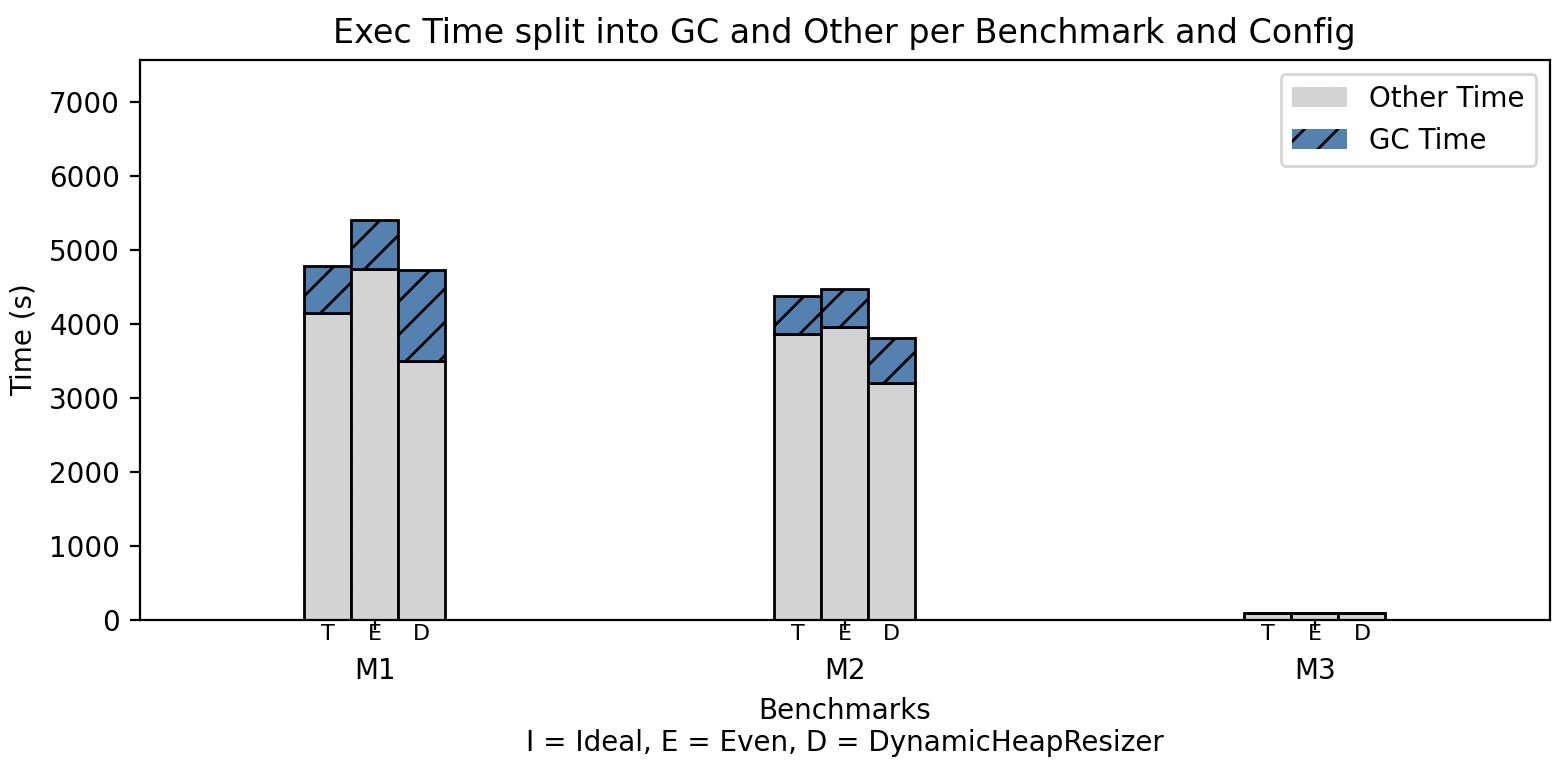
\includegraphics[width=1\columnwidth]{fig/eval_graph.png}
  \caption{Execution time and GC time comparisons}
  \label{fig:gc_exec_time}
\end{figure}

\subsection{Page Cache Usage and Device Traffic}

In this subsection, we analyze the page cache utilization under the Dynamic Heap Resizer
(DHR) for the three evaluated workloads: M1, M2, and M3. Figure~\ref{fig:pc_dhr} 
illustrates the page cache usage over time demonstrates different caching behaviors, 
adapting to each benchmark and their distinct memory access patterns and working set sizes.

For M1, the page cache usage increases rapidly during the initial phase of execution, 
stabilizing at approximately 17.6~GB. This indicates that M1 aggressively utilizes 
the page cache early on, due to frequent and repeated accesses.
After the initial rise, the flat line shows that M1's data fits in the page cache, so later accesses have less I/O delay.
M2, exhibits a more gradual increase in page cache usage, 
eventually reaching a similar final usage level of around 17.5~GB.
This slower increase is due to the workload consisting of more distributed 
data accesses, taking longer to populate the page cache fully. This 
indicates that M2 patterns require more time to reach an optimal cache utilization.
M3 shows periodic drops and rises, indicating batching behavior with bursts of cache usage between processing phases.

Overall, these results indicate that the Dynamic Heap Resizer effectively manages DRAM allocation to maximize page
cache utility for workloads that benefit from dynamic partitioning at runtime. 

\begin{figure}[htbp]
  \centering
  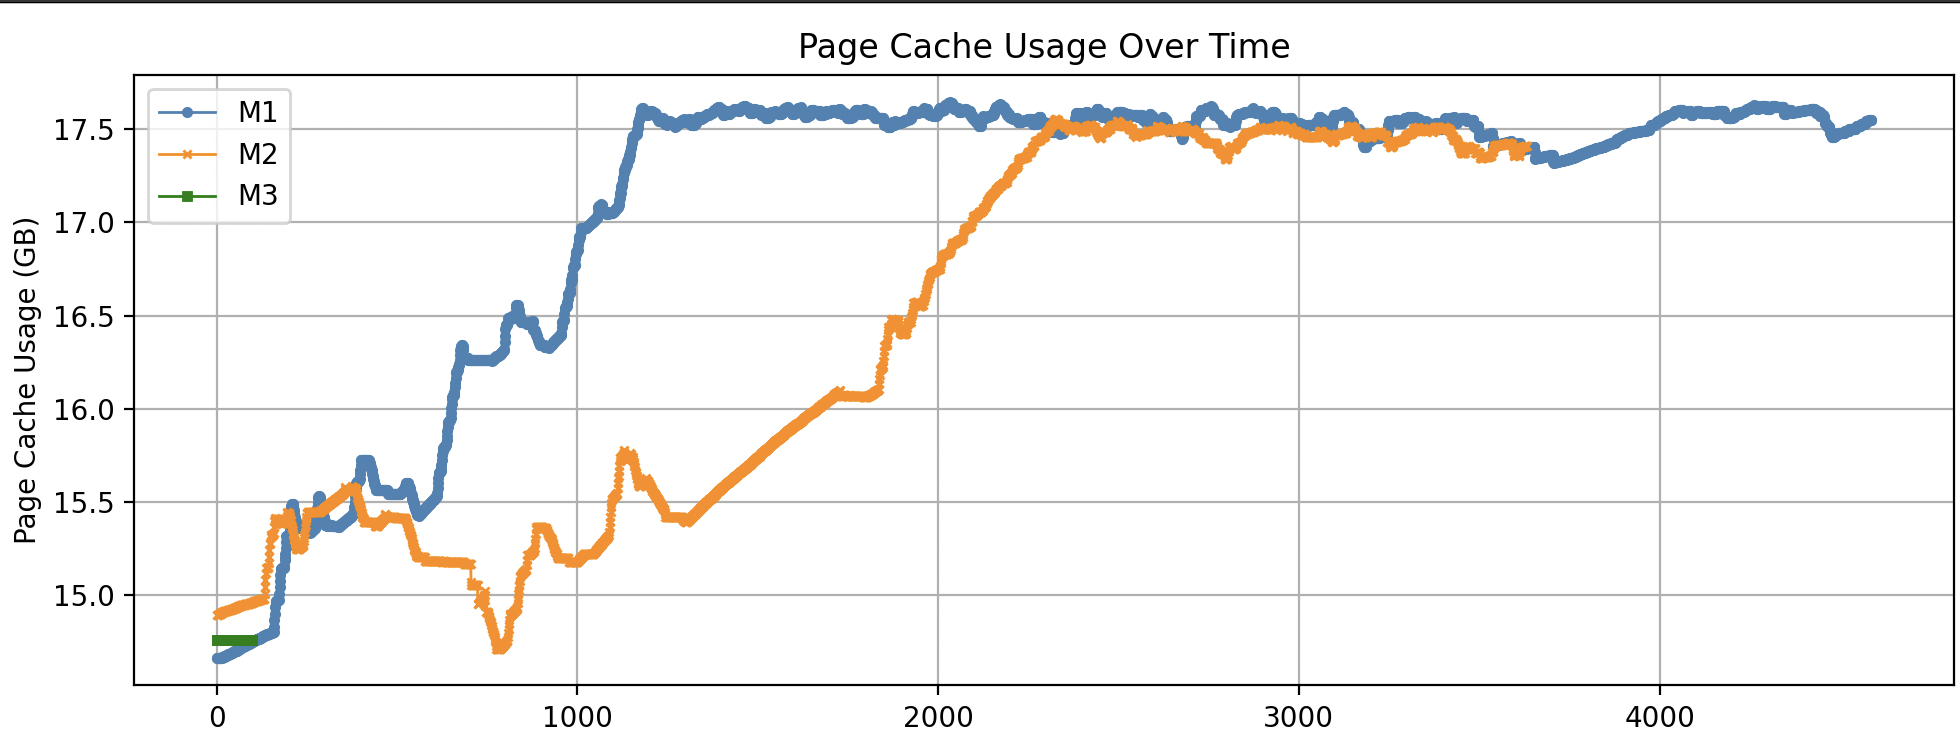
\includegraphics[width=1\columnwidth]{fig/pagecache_dhr.png}
  \caption{Page cache usage with Dynamic Heap Resizing, for M1, M2, M3 benchmarks}
  \label{fig:pc_dhr}
\end{figure}

\begin{table}[h]
\centering
\caption{Average read and write traffic (MB/s) for each benchmark under Ideal, Even, and DHR configurations.}
\label{tab:traffic}
\begin{tabular}{l|ccc|ccc}
\hline
 & \multicolumn{3}{c|}{Read (MB/s)} & \multicolumn{3}{c}{Write (MB/s)} \\
Config & M1 & M2 & M3 & M1 & M2 & M3 \\
\hline
Ideal & 0.07 & 0.07 & 0.002 & 22.79 & 22.59 & 0.01 \\
Even  & 0.07 & 0.07 & 0.002 & 20.80 & 21.24 & 0.01 \\
DHR   & 0.07 & 0.08 & 0.002 & 24.80 & 28.06 & 0.05 \\
\hline
\end{tabular}
\end{table}

\subsection{Query Throughput (QPS) Analysis}

Figure~\ref{fig:qps_plot}: Compares Queries per second (QPS) for each benchmark (M1, M2, M3)
under Ideal, Even, and Dynamic Heap Resizer (DHR) configurations.

In this plot, we observe that for M1, DHR achieves the highest QPS compared to both 
Ideal and Even configurations, indicating that dynamically adapting the heap provides
benefits for this workload. For M2, DHR again slightly outperforms both Ideal and Even, 
showing that its adjustments handle the memory and I/O requirements effectively. In M3,
however, DHR achieves slightly lower QPS compared to Ideal, but remains higher than the
Even configuration. This minor difference suggests that the Dynamic Heap Resizer’s gradual 
adjustments cannot resize aggressively enough during batched phases.
Overall, DHR shows improved or comparable QPS across benchmarks, demonstrating its ability 
to adapt efficiently to varying workload characteristics.

\begin{figure}[htbp]
  \centering
  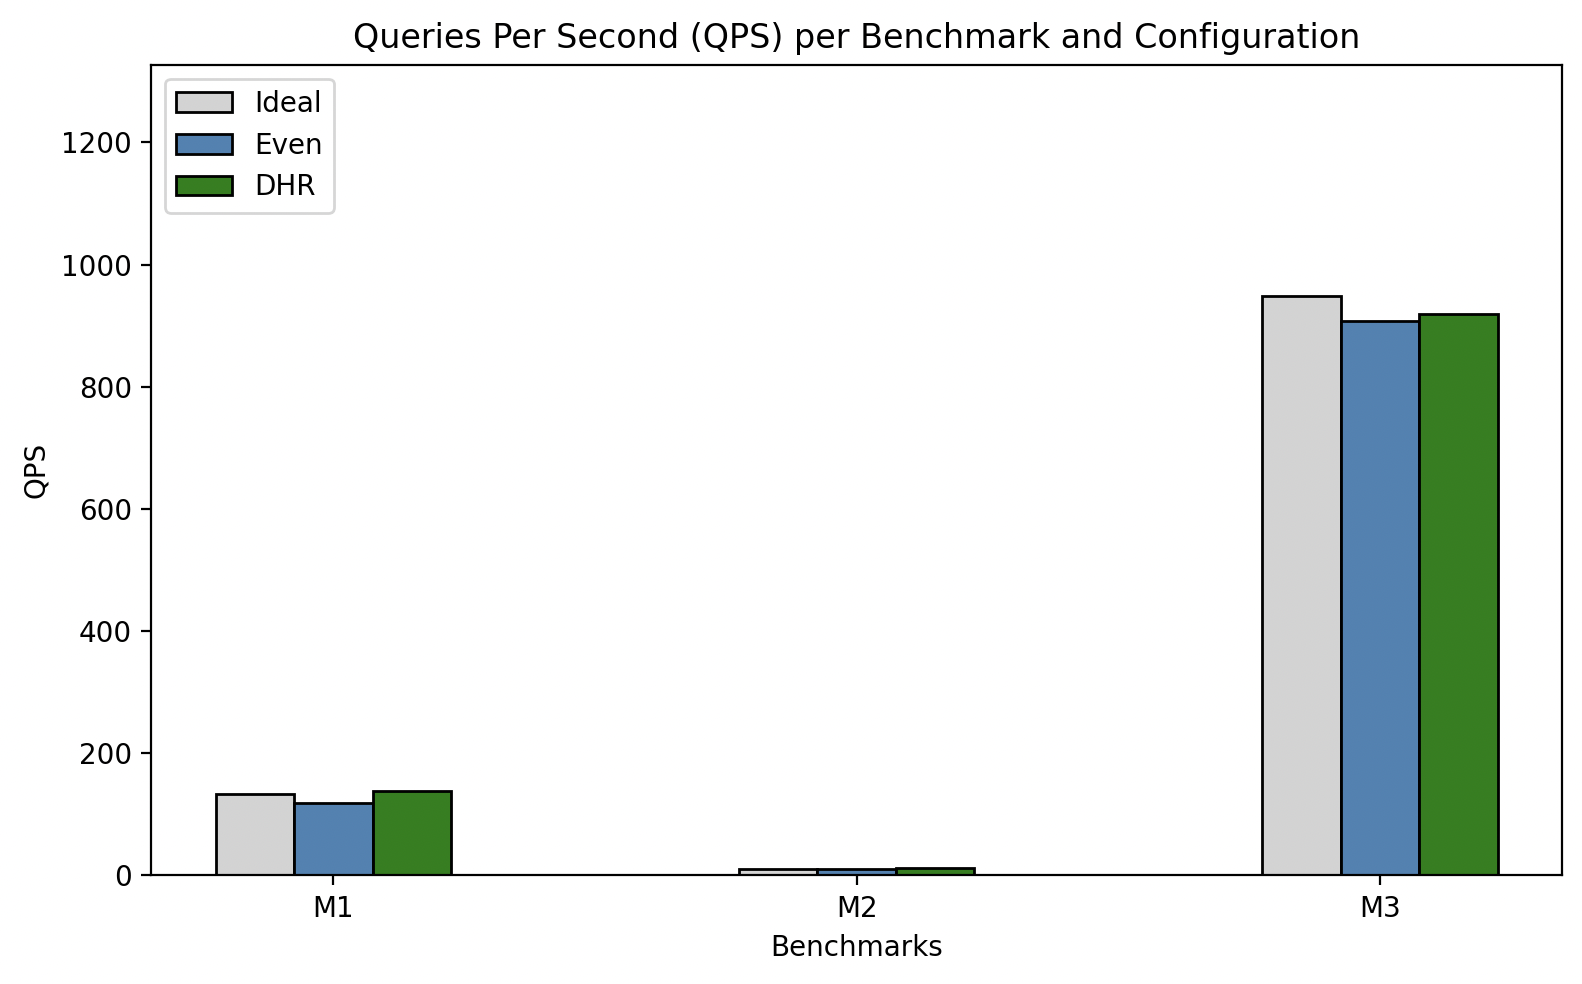
\includegraphics[width=1\columnwidth]{fig/qps_plot.png}
  \caption{Queries per second (QPS) for benchmarks M1, M2, and M3}
  \label{fig:qps_plot}
\end{figure}

